\documentclass[11pt,twoside]{article}

\usepackage{amsmath}
\usepackage{amssymb}
\usepackage{amsthm}
\usepackage{courier} % Required for the courier font
\usepackage{extramarks} % Required for headers and footers
\usepackage{fancyhdr} % Required for custom headers
\usepackage{graphicx} % Required to insert images
\usepackage{lastpage} % Required to determine the last page for the footer
\usepackage{listings} % Required for insertion of code
\usepackage{lipsum} % Used for inserting dummy 'Lorem ipsum' text into the template
\usepackage{mathtools}
\usepackage{subcaption}

\usepackage[margin=1in]{geometry}
\usepackage[usenames,dvipsnames]{color} % Required for custom colors

\usepackage{color}

\definecolor{mygreen}{rgb}{0,0.6,0}
\definecolor{mygray}{rgb}{0.5,0.5,0.5}
\definecolor{mymauve}{rgb}{0.58,0,0.82}

\lstset{ %
  commentstyle=\color{mygreen},    % comment style
  frame=single,	                   % adds a frame around the code
  keywordstyle=\color{blue},       % keyword style
  language=Python,                 % the language of the code
  numbers=left,                    % where to put the line-numbers; possible values are (none, left, right)
  numbersep=5pt,                   % how far the line-numbers are from the code
  numberstyle=\tiny\color{mygray}, % the style that is used for the line-numbers
  stringstyle=\color{mymauve},     % string literal style
}

\begin{document}

\title{CSC411 - Project \#4}
\author{Yui Chit (Michael) Wong - 999806232\\Yijin (Catherine) Wang - 998350476}
\maketitle

\clearpage

\section*{Part 1}
\paragraph{Question}
Explain precisely why the code corresponds to the pseudocode below. Specifically, in your report, explain how all the terms ( $G_t$ , $\pi$ , and the update to $\theta$ ) are computed, quoting the relevant lines of Python.

\begin{figure*}[h]
	\centering
	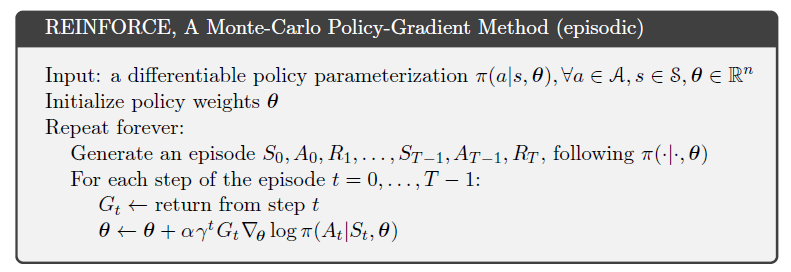
\includegraphics[scale=0.8]{sutton&barto.png}
	\caption*{Pseudocode}
\end{figure*}

\paragraph{Answer}
As mentioned on the assignment page, the policy function $\pi_{\theta}$ is implemented with a single-hidden-layer of neural network. Since the actions for the bipedal walker is continuous, we have to use a Gaussian distribution on $\pi$. Thus we pass the hidden layer into two separately fully connected output, which represents the $\mu$ and $\sigma$ to the normal distribution. The activation function are $tanh$ and $softplus$ (variation on $ReLU$) respectively. The $sigma$ value are also clipped if it is too small or big.

\begin{lstlisting}
# 1 layer of hidden unit. Activation is ReLU
hidden = fully_connected(
    inputs=x,
    num_outputs=hidden_size,
    activation_fn=tf.nn.relu,
    weights_initializer=hw_init,
    weights_regularizer=None,
    biases_initializer=hb_init,
    scope='hidden')

# use last layer of neural network as phi(a, s) (the feature)
# mu = phi(s, a)^T dot theta
mus = fully_connected(
    inputs=hidden,
    num_outputs=output_units,
    activation_fn=tf.tanh,
    weights_initializer=mw_init,
    weights_regularizer=None,
    biases_initializer=mb_init,
    scope='mus')

# softplus is similar to ReLU. Activation function is g(x) = ln(1+e^x)
sigmas = tf.clip_by_value(fully_connected(
    inputs=hidden,
    num_outputs=output_units,
    activation_fn=tf.nn.softplus,
    weights_initializer=sw_init,
    weights_regularizer=None,
    biases_initializer=sb_init,
    scope='sigmas'),
    TINY, 5)
\end{lstlisting}

As for the weight intialization, if there is no weight saved from the previous run, we will initialize the weight $\theta$. There are one $w$ and $b$ for each of the layers (hidden, $\mu$, $\sigma$). When initializing the weight to each layer, the program uses $xavier initialization$, another variation of random weight initialization that keep the scale of the gradients in roughly the same scale.

\begin{lstlisting}
# if we have the w's and b's saved, load it. Otherwise initialize it
if args.load_model:
    model = np.load(args.load_model)
    hw_init = tf.constant_initializer(model['hidden/weights'])
    hb_init = tf.constant_initializer(model['hidden/biases'])
    mw_init = tf.constant_initializer(model['mus/weights'])
    mb_init = tf.constant_initializer(model['mus/biases'])
    sw_init = tf.constant_initializer(model['sigmas/weights'])
    sb_init = tf.constant_initializer(model['sigmas/biases'])
else:
    hw_init = weights_init
    hb_init = relu_init
    mw_init = weights_init
    mb_init = relu_init
    sw_init = weights_init
    sb_init = relu_init
\end{lstlisting}

Once everything is initialized, we will start training. For each iteration, we will reset the environment (line 2), then generate the states, actions, and rewards from time 0 to time $T$. When generating the actions, we will randomly sample from the $\pi$ normal distribution (line 16). Then based on the $pi.sample()$, we will generate the corresponding action $pi_sample$, and using the action, the new state, reward would be generated. We will keep track of all the states, actions, and rewards in 3 lists ($ep\_states, ep\_actions, $ and $ep\_rewards$). We will also keep track of the total discounted rewards using the variable $G$ (line 20). Then to obtain $G_t$, the discounted reward starting from time t, the program calls a culmulation sum function on the $ep_rewards$ then subtract it from $G$ (line 30). Thus $returns$ would be storing the total discouned rewards for each time from time 0 to $T-1$.

\begin{lstlisting}
for ep in range(16384):
    obs = env.reset()	# reset the environment

    G = 0	    # generating all the states and actions and rewards
    ep_states = []
    ep_actions = []
    ep_rewards = [0]
    done = False
    t = 0
    I = 1
    while not done:
        ep_states.append(obs)
        env.render()
        # pi.sample() is the list of randomly generated probablity
        # pi_sample becomes the action
        action = sess.run([pi_sample], feed_dict={x:[obs]})[0][0]
        ep_actions.append(action)
        obs, reward, done, info = env.step(action)
        ep_rewards.append(reward * I)
        G += reward * I # G is the total discounted reward
        I *= gamma

        t += 1
        if t >= MAX_STEPS:
            break
    # done generating

    if not args.load_model:
        # G_t = total - culmulative up to time t. 
        returns = np.array([G - np.cumsum(ep_rewards[:-1])]).T
        index = ep % MEMORY
        
        # ep_states contains all the state S_0 to S_T-1
        # ep_actions contains all the actions from A_0 to A_T-1
        # returns (ie reward) contains all the G_t's form t=0 to t=T
        _ = sess.run([train_op],
                    feed_dict={x:np.array(ep_states),
                                y:np.array(ep_actions),
                                Returns:returns })
\end{lstlisting}

Then we will pass the list of states, actions, and the returns into the training step (line 36-39). Then tensorflow will use the state and the weights to generate a new $\mu$ and $\sigma$. Then it will compute the log probability of the actions given the generate $\mu$ and $\sigma$. 

\begin{lstlisting}
# log probability of y given mu and sigma
log_pi = pi.log_prob(y, name='log_pi')
\end{lstlisting}

The cost function used is $J(\theta) = -\sum[G_t log \pi (A_t | S_t, \theta)]$. The program uses gradient descent to adjust the $\theta$ to minimize the cost function

\begin{lstlisting}
# Returns is a 1 x (T-1) array for float (rewards)
Returns = tf.placeholder(tf.float32, name='Returns')
optimizer = tf.train.GradientDescentOptimizer(alpha)
train_op = optimizer.minimize(-1.0 * Returns * log_pi)
\end{lstlisting}

\clearpage



\section*{Part 2}

\paragraph{Question}

\paragraph{Answer}

\clearpage



\section*{Part 3}

\paragraph{Question}

\paragraph{Answer}

\clearpage



\end{document}